\documentclass{homework}
\usepackage{xcolor}
\usepackage{nicematrix}
\usepackage{booktabs}
\usepackage{enumitem}
\usepackage{caption}
\usepackage{subcaption}
\usepackage{leftidx}

\NiceMatrixOptions{cell-space-limits = 1pt}

\title{Solutions Excercise 1}
\author{
  Maksimov, Dmitrii\\
  \texttt{dmitrii.maksimov@fau.de}
  \and
  Ilia, Dudnik\\
  \texttt{ilia.dudnik@fau.de}
}

\begin{document}

\maketitle

\exercise
\begin{enumerate}[label=(\alph*)]
	\item State the dual program corresponding to the following linear programs:
	\begin{align*}
		\text{max} \quad
		&c^T x + d^T y \\
		\text{s.t.} \quad
		&Ax \geq b \\
		&g^T y = f \\
		&x, y \geq 0
	\end{align*}
	Here, $f \in \R, c \in \R^n, b \in \R^m, d,g \in \R^l \text{ and } A \in \R^{m \times n}$.

	Following to the general rules for finding the dual of a given linear program, the corresponding dual program:
		\begin{align*}
			\text{min} \quad
			&b^T u + f\cdot v \\
			\text{s.t.} \quad
			&A^T u \geq c \\
			&g\cdot v \geq d \\
			&u \leq 0
		\end{align*}
	\item Use Part (a) in order to show or disprove that $(x^\star, y^\star) = (\frac{13}{3}, 0, \frac{5}{3}, 1, 0)^T$ is an optimal solution for
		\begin{align*}
			\text{max} \quad
			&(6, -1, -3) x + (4, -6)y \\
			\text{s.t.} \quad
			&\begin{pmatrix}
			-2 & -1 & \frac{17}{5} \\
			-1 & 1 &-1
			\end{pmatrix}x \geq  \begin{pmatrix}
							-3 \\
							-6
							\end{pmatrix}\\
			&(2, -3)y = 2 \\
			&x,y, \geq 0
		\end{align*}

		Using python and SciPy check whether $(x^\star, y^\star) = (\frac{13}{3}, 0, \frac{5}{3}, 1, 0)^T \text{ is an optimal solution and } W^\star = Z^\star$. The code implementation can be founded here \href{https://colab.research.google.com/drive/183PlRiFx1C_aDkJ0yZC86WoozAwRDpcC?usp=sharing}{Code}. Due to SciPy restrictions linear function to be minimized: $-Z = -c^T x - d^T y$
\newpage
\begin{figure}[hbt!]
	\centering
	
\includegraphics[width=0.8\textwidth]{primal_solution.png}
	\caption{Solution of primal problem}
\end{figure}

	As we can see $x = (4.3, 0, 1.6, 1., 0.)^T =  (x^\star, y^\star) = (\frac{13}{3}, 0, \frac{5}{3}, 1, 0)^T \text{ and } Z^\star = 25$.

	Now, solve the dual problem

\begin{figure}[hbt!]
	\centering
	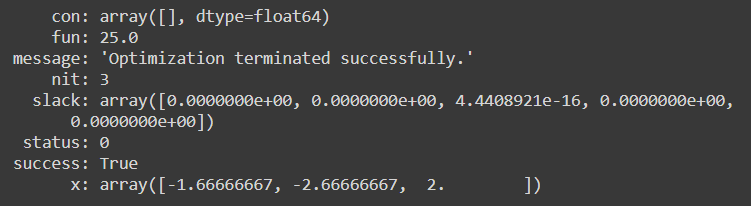
\includegraphics[width=0.8\textwidth]{dual_solution.png}
	\caption{Solution of dual problem}
\end{figure}
	Since $W^\star = Z^\star$ and all above mentioned $(x^\star, y^\star) = (\frac{13}{3}, 0, \frac{5}{3}, 1, 0)^T$ is an optimal solution.
\end{enumerate}
\exercise
Consider the following program:
\begin{align*}
	\text{max} \quad
	&7x_1 + 6x_2 + 5x_3 - 2x_4 + 3x_5\\
	\text{s.t.} \quad
	&x_1 + 3x_2 + 5x_3 - 2x_4 + 2x_5\leq 4 \\
	&4x_1 + 2x_2 - 2x_3 + x_4 + x_5\leq 3 \\
	&2x_1 + 4x_2 + 4x_3 - 2x_4 + 5x_5\leq 5 \\
	&3x_1 + x_2 + 2x_3 - x_4 - 2x_5\leq 1 \\
	&x_1, \dots, x_5 \geq 0
\end{align*}
\begin{enumerate}[label=(\alph*)]
	\item Formulate the corresponding dual program

	Following to the general rules for finding the dual of a given linear program, the corresponding dual program:
	\begin{align*}
		\text{min} \quad
		&4y_1 + 3y_2 + 5y_3 + y_4\\
		\text{s.t.} \quad
		&y_1 + 4y_2 + 2y_3 + 3y_4\geq 7 \\
		&3y_1 + 2y_2 + 4y_3 + y_4\geq 6 \\
		&5y_1 - 2y_2 + 4y_3 + 2y_4\geq 5 \\
		&-2y_1 + y_2 - 2y_3 - y_4\geq -2 \\
		&2y_1 + y_2 +5 y_3 - 2y_4\geq 3 \\
		&y_1, \dots, y_4 \geq 0
	\end{align*}
	\item Check if $x^\star = (0, \frac{4}{3}, \frac{2}{3}, \frac{5}{3}, 0)^T$ is an optimal solution via the complementary slackness theorem.
	
	\begin{itemize}
	\item 1 constraint: $0 + 4 + \frac{10}{3} - \frac{10}{3} + 0 \leq 4 \Rightarrow 4 \leq 4 \rightarrow \text{tight}$
	\item 2 constraint: $0 + \frac{8}{3} - \frac{4}{3} + \frac{5}{3} + 0 \leq 3 \Rightarrow 3 \leq 3 \rightarrow \text{tight}$
	\item 3 constraint: $0 + \frac{16}{3} + \frac{8}{3} - \frac{10}{3} + 0 \leq 5 \Rightarrow \frac{14}{3} \leq 5 \rightarrow \text{slack}$
	\item 4 constraint: $0 + \frac{4}{3} + \frac{4}{3} - \frac{5}{3} + 0 \leq 1 \Rightarrow 1 \leq 1 \rightarrow \text{tight}$
	\item $x_i^\star \geq 0 \text{ for } i \in [1, \dots, 5]$
	\end{itemize}

	Hence, $y_1, y_2, y_4 \geq 0, y_3 = 0$.
	
	Since $x_2, x_3, x_4 > 0$, complementary slackness demand that the corresponding constraints should be tight. Putting this together:
	\[
	\begin{cases} 
		3y_1^\star + 2y_2^\star + y_4^\star = 6 \\
		5y_1^\star - 2y_2^\star + 2y_4^\star = 5 \\
		-2y_1^\star + y_2^\star - y_4^\star = -2 
	\end{cases}
	\]
	$y^\star = (1, 1, 0, 1)$.
	Check whether $y^\star$ satisfies the dual feasibility conditions:
	\begin{itemize}
	\item $y_i^\star \geq 0 \text{ for } i \in [1, \dots, 4]$
	\item 1 constraint: $1 + 4 + 3\geq 7$ - yes
	\item 5 constraint: $2 + 1 - 2\geq 3$ - no
	\end{itemize}
	It is, so (1, 1, 0, 1) is infeasible $\Rightarrow x^\star$ is not an optimal primal solution. 
	
\end{enumerate}

\end{document}